
\subsection{Where do additional funds go?}%
\label{sub:where_do_additional_funds_go_}

\begin{itemize}
    \item Above we find that app use reduces discretionary spend but does not
        increase flows into savings accounts.

    \item This begs the question: ``Where does the money go?``

    \item One possibility is that people do save more but that the additional
        savings go into either long-term investment accounts that cannot be
        linked to the app (e.g. accounts at Vanguard or other investment
        services) or into conventional savings accounts that people users do
        not link to the app. Check for additional outgoing transfers to
        investment services and transfers into accounts that are not added to
        app.

    \item I first look at flows into investment accounts.

    \item Then at transfers from current accounts. Here I consider two metrics.
        First, savings defined by users, second, total transfers.

    \item Another possibility is that people pay down debt. Can check whether
        payments into credit card accounts or repayment of loands increases.

    \item Here, I first look at flows into credit card accounts.

    \item Then at loan repayments. Control for loan takeout. Actually, plot
        separately, then control for takeout in repayment in case there is a
        pattern.
\end{itemize}

\begin{figure}[H]
    \centering
    \caption{Money flows}%
    \label{fig:int_ext_results}
    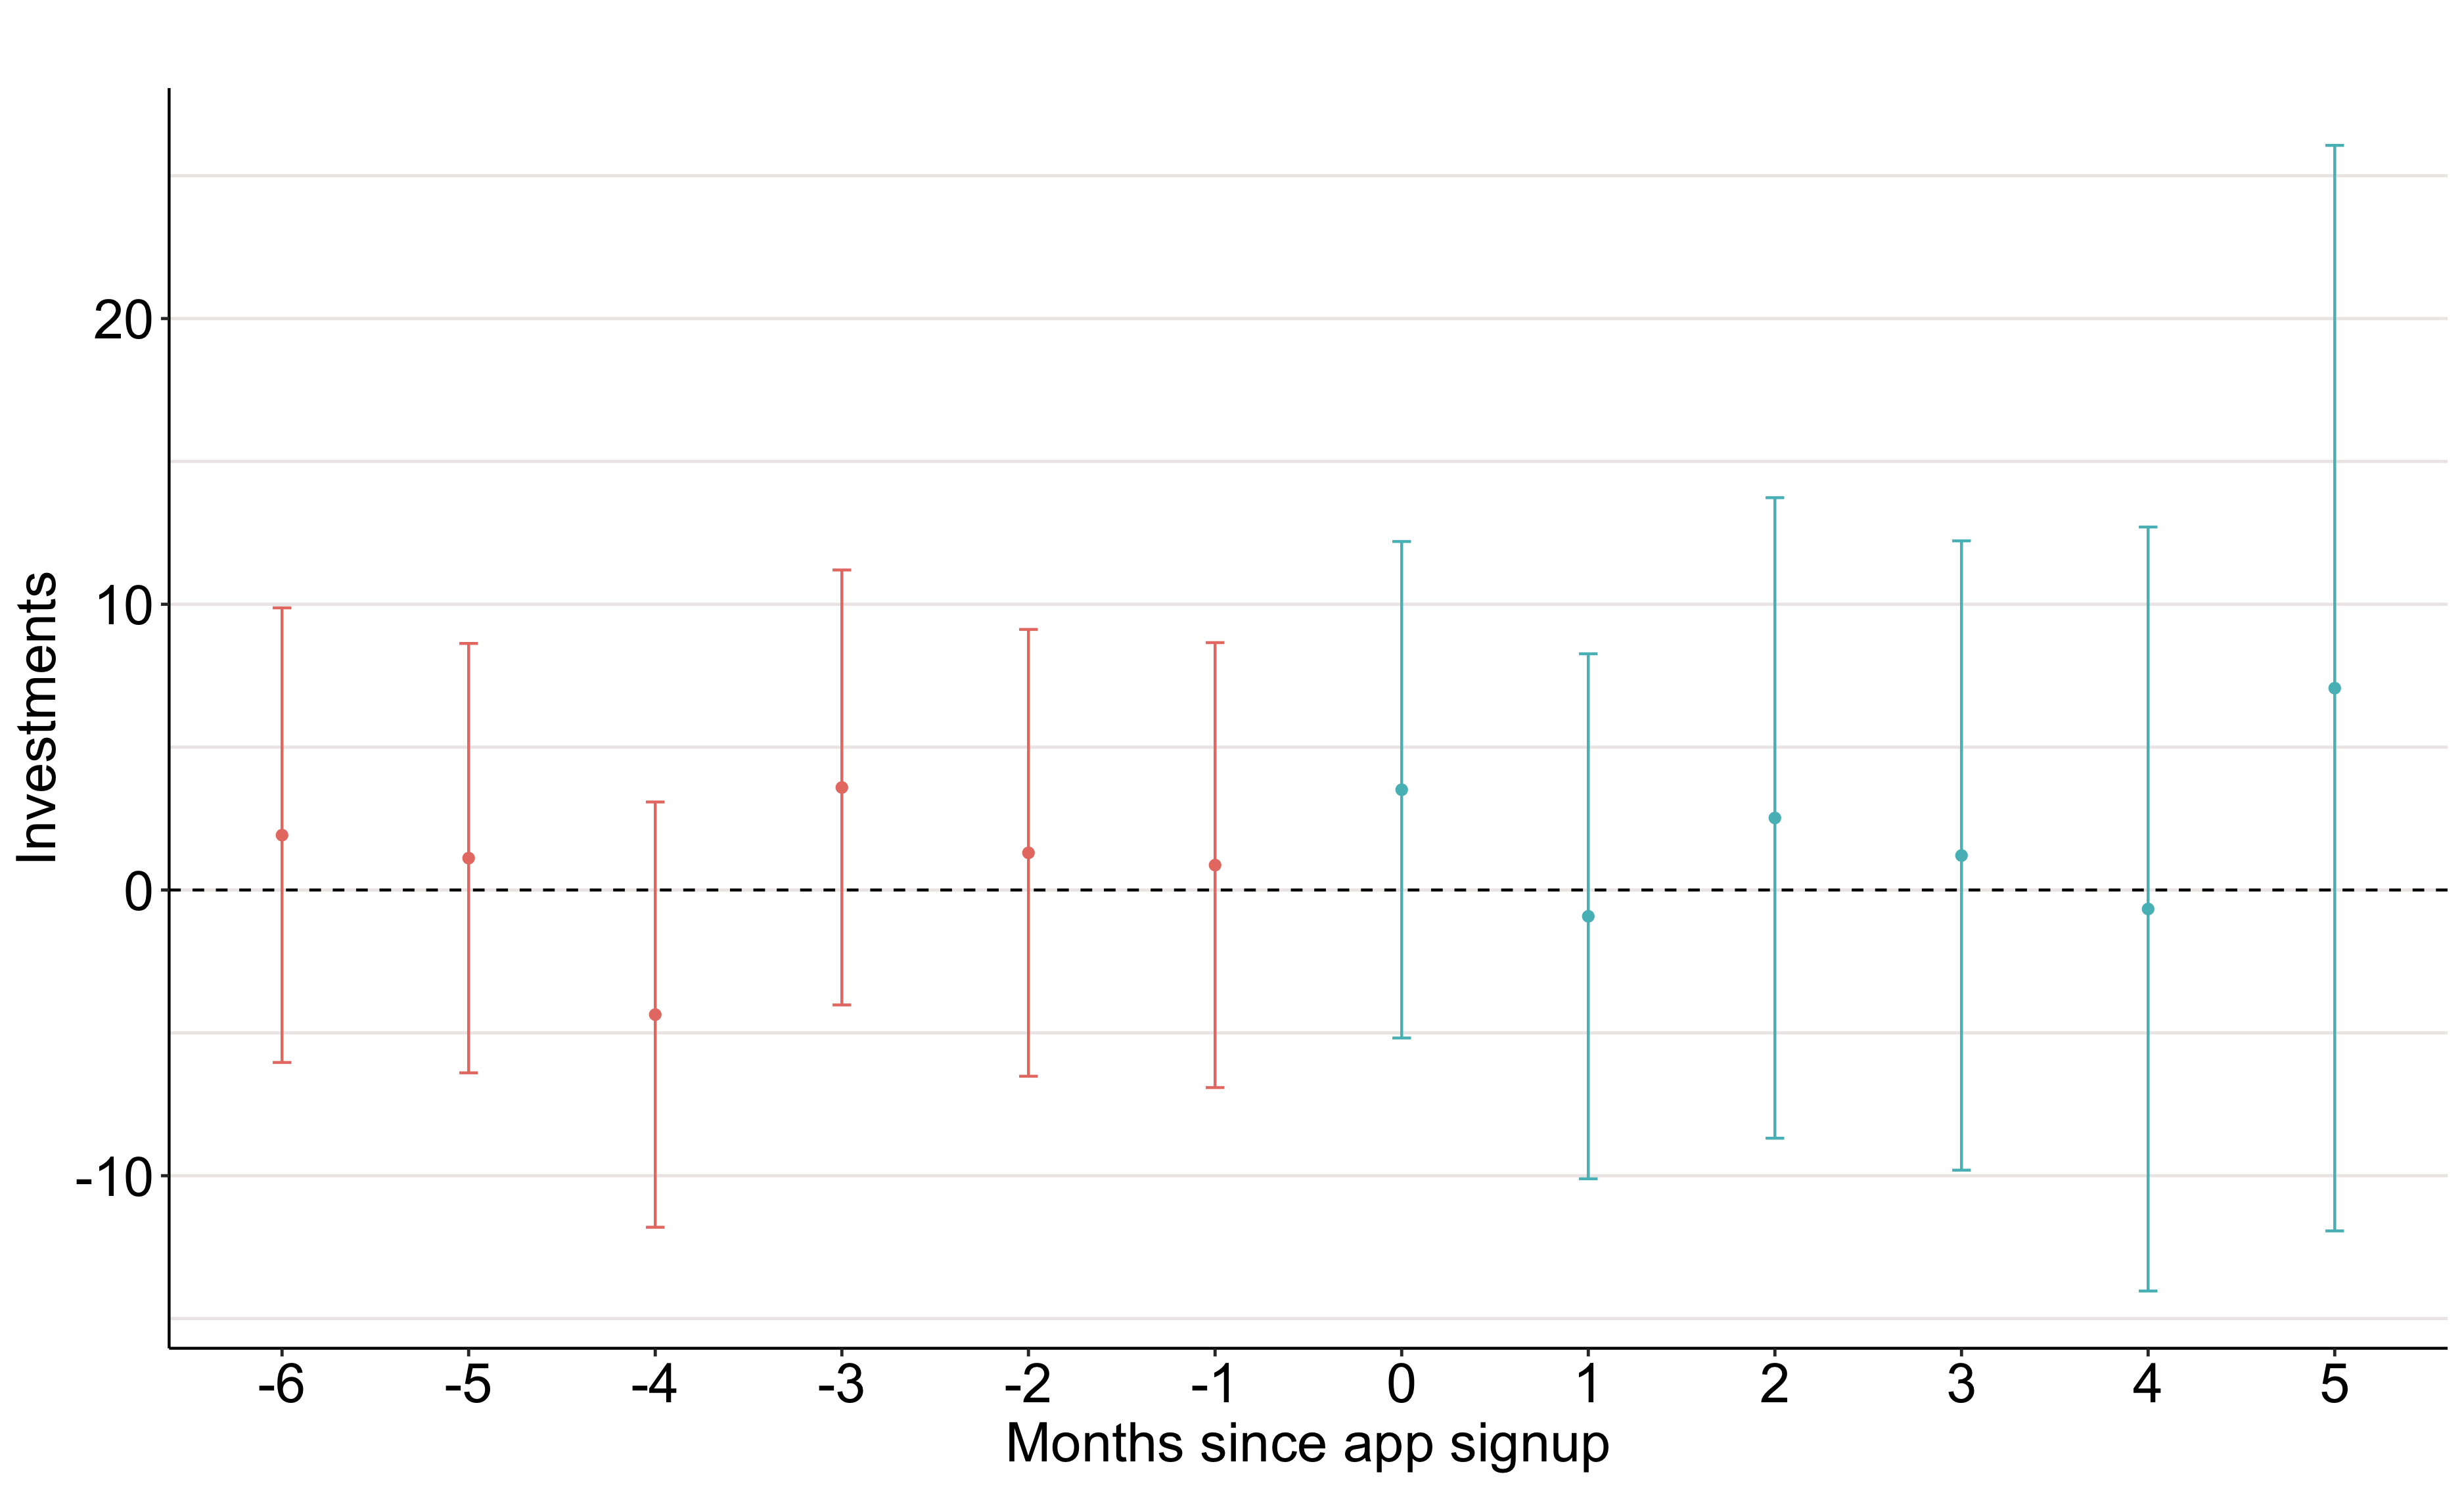
\includegraphics[width=.49\textwidth]{\figdir/investments_cond_es.png}
    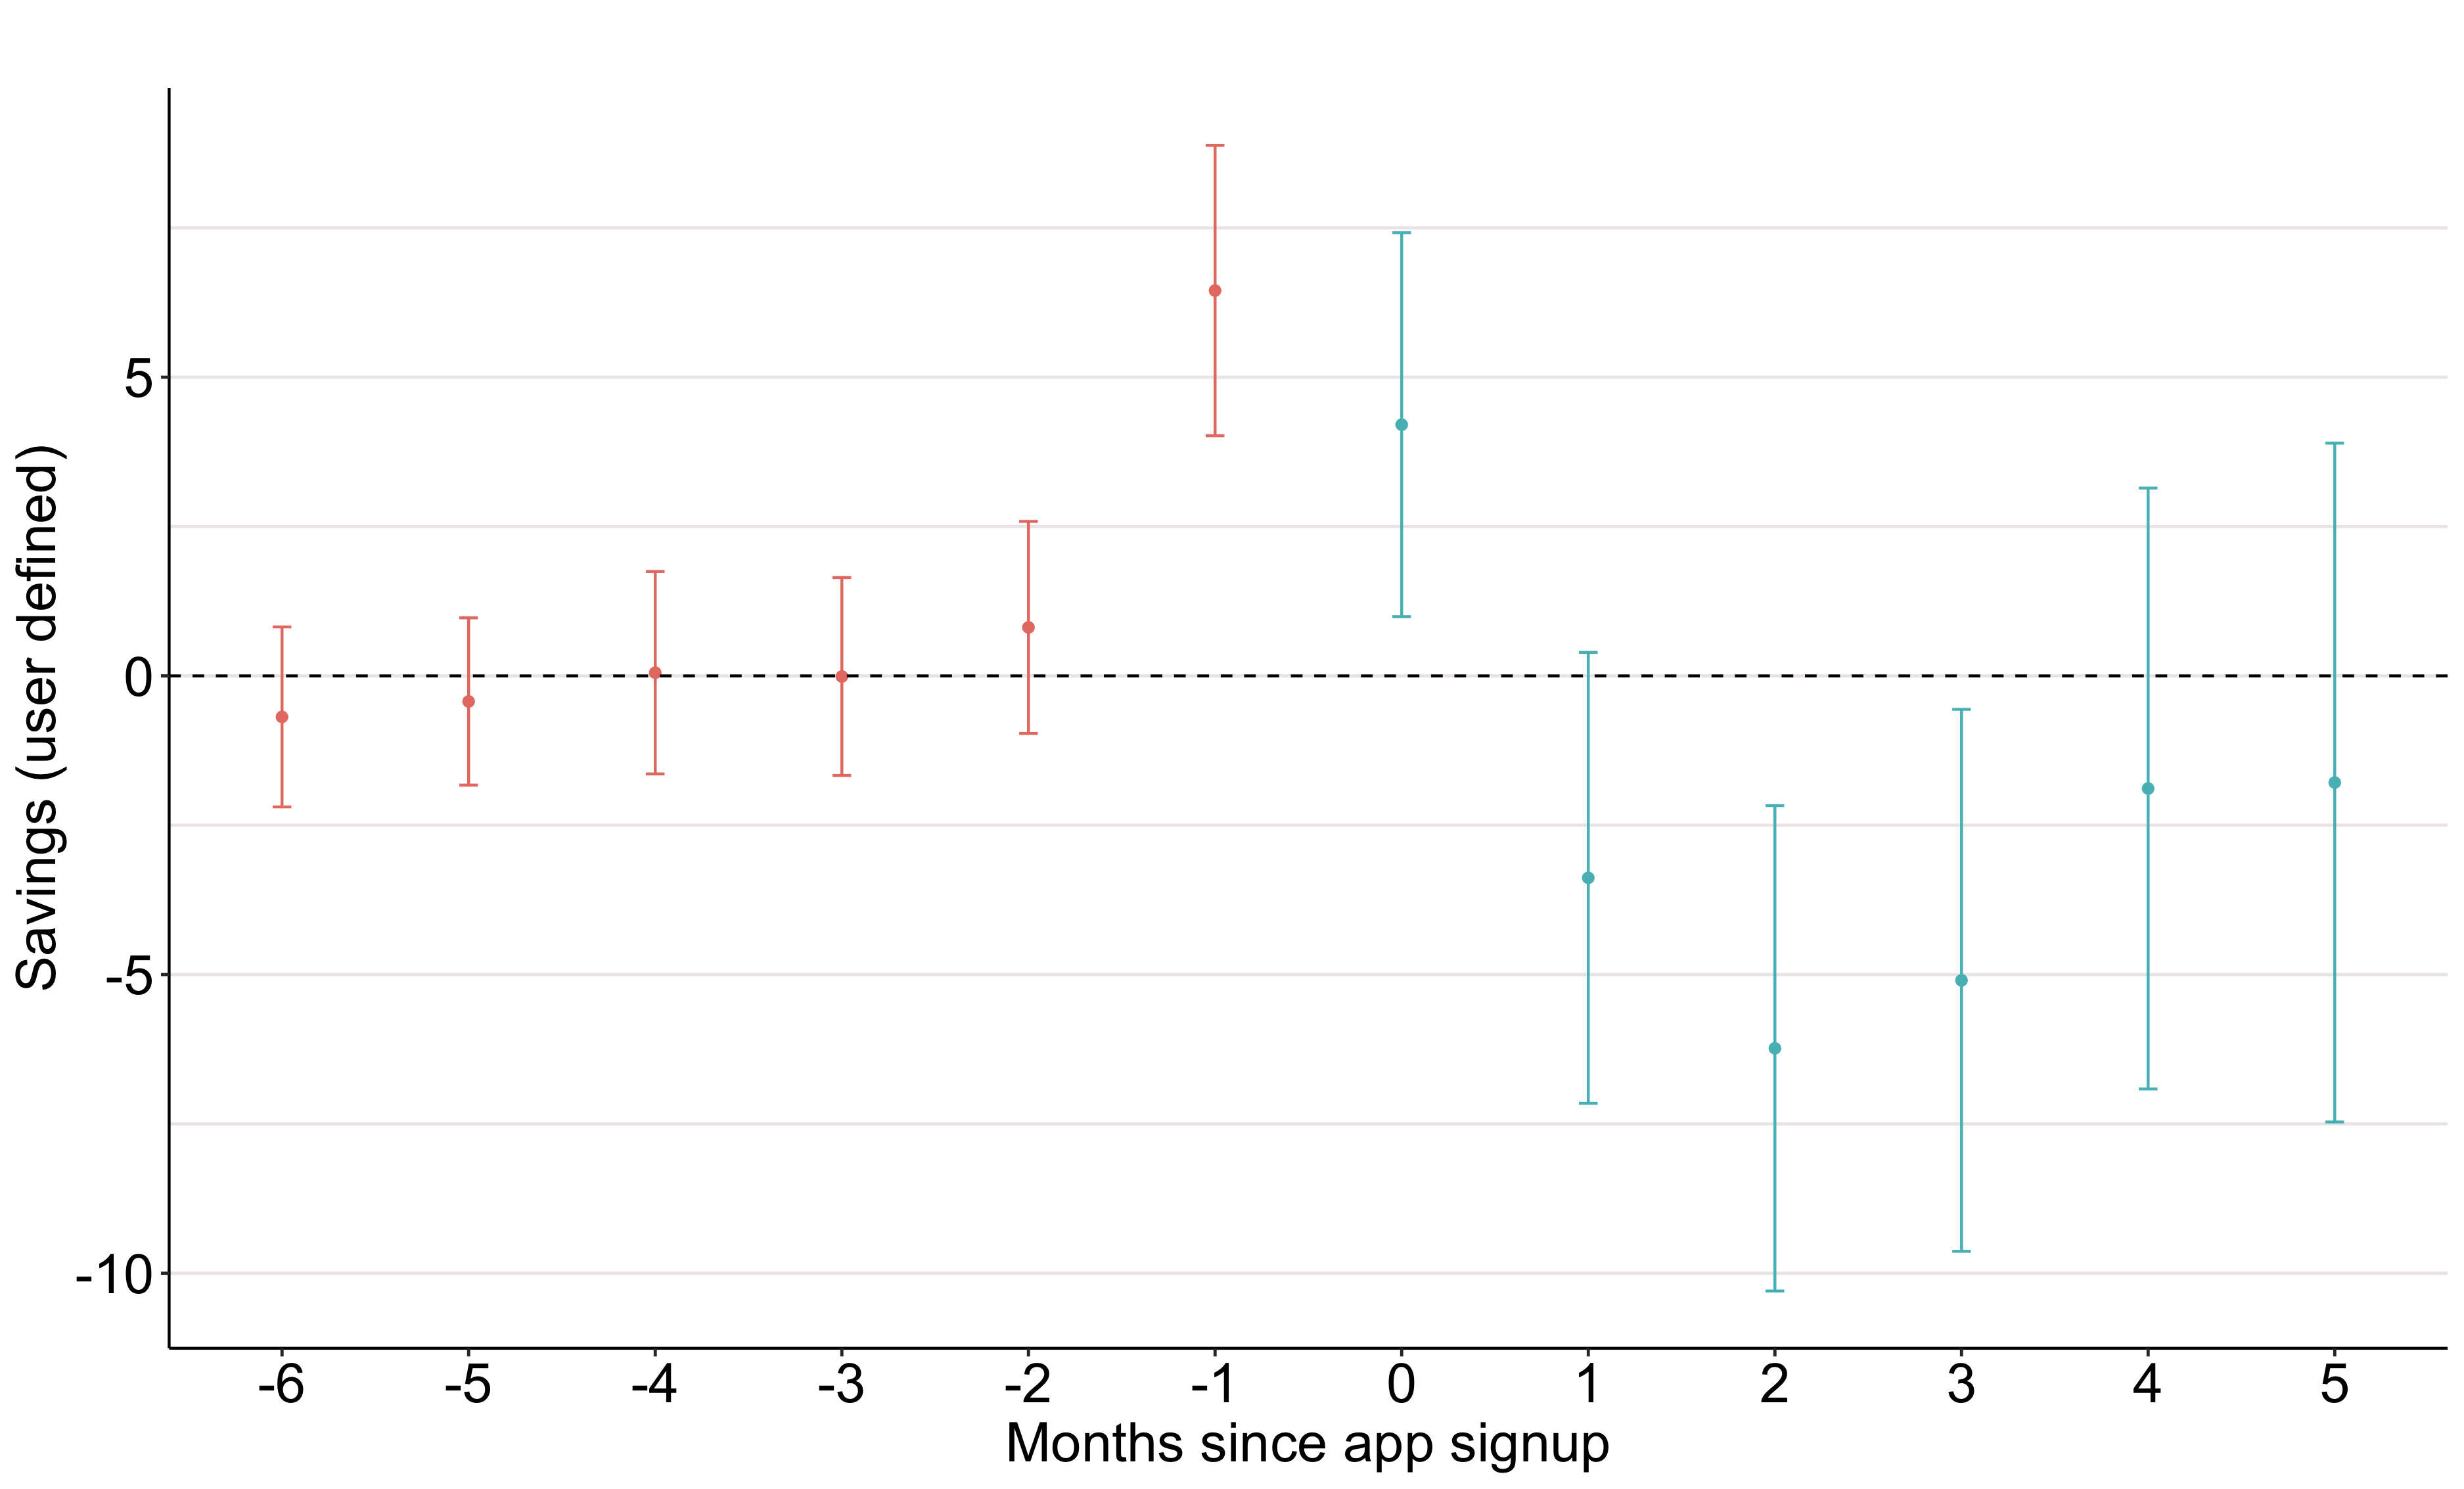
\includegraphics[width=.49\textwidth]{\figdir/up_savings_cond_es.png}
    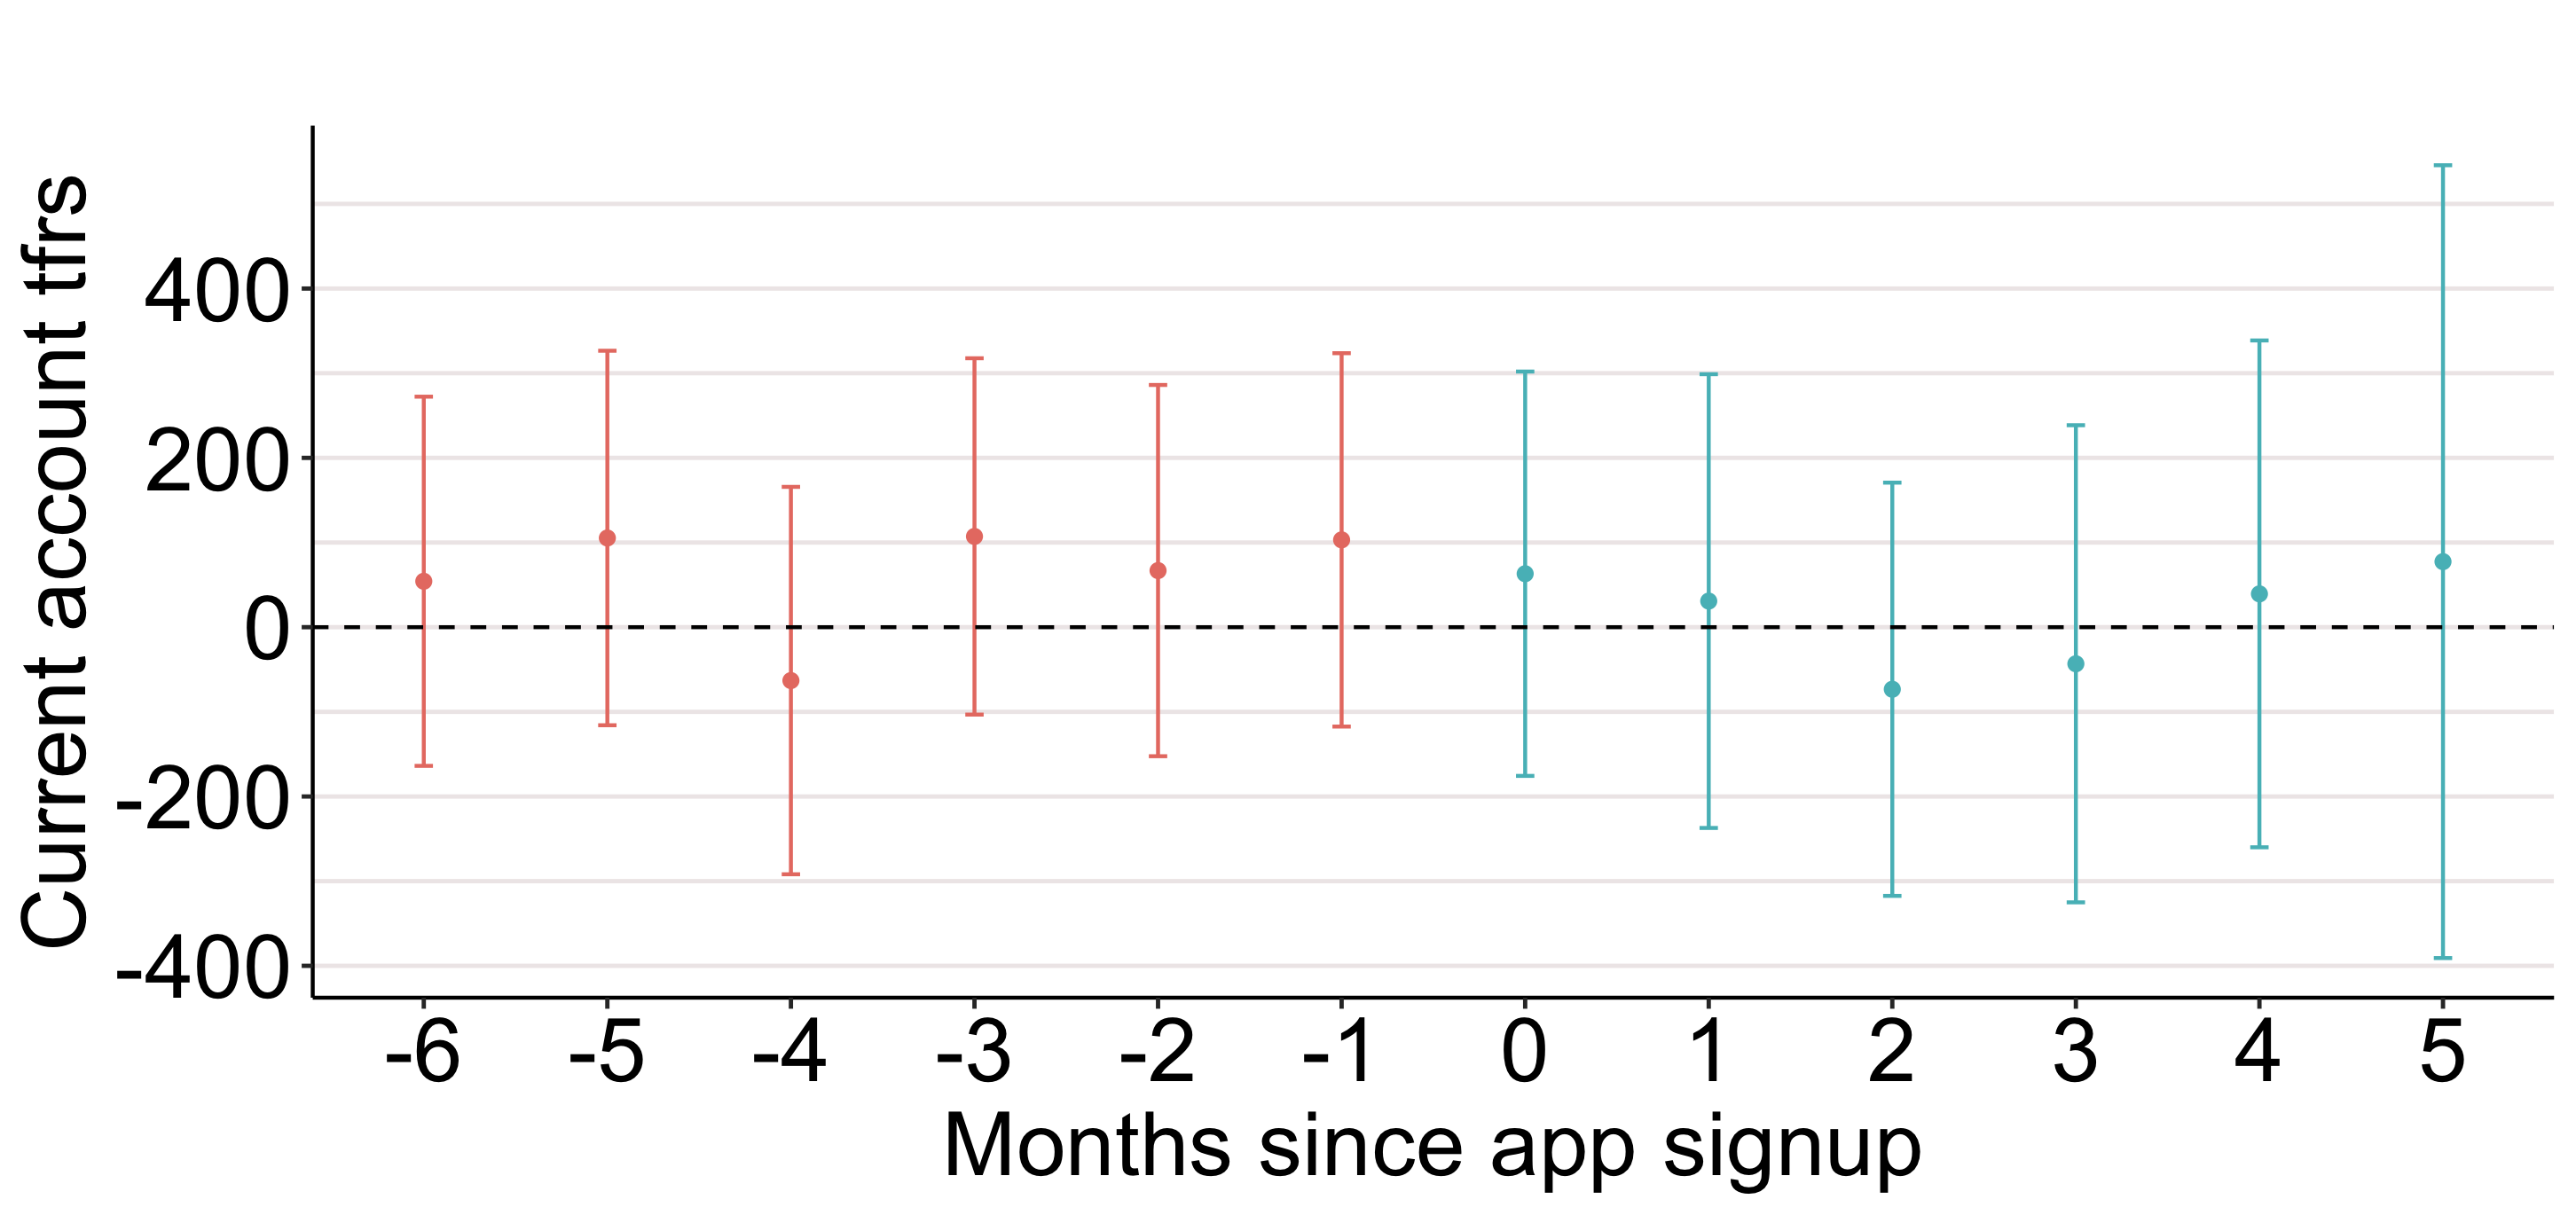
\includegraphics[width=.49\textwidth]{\figdir/ca_transfers_cond_es.png}
    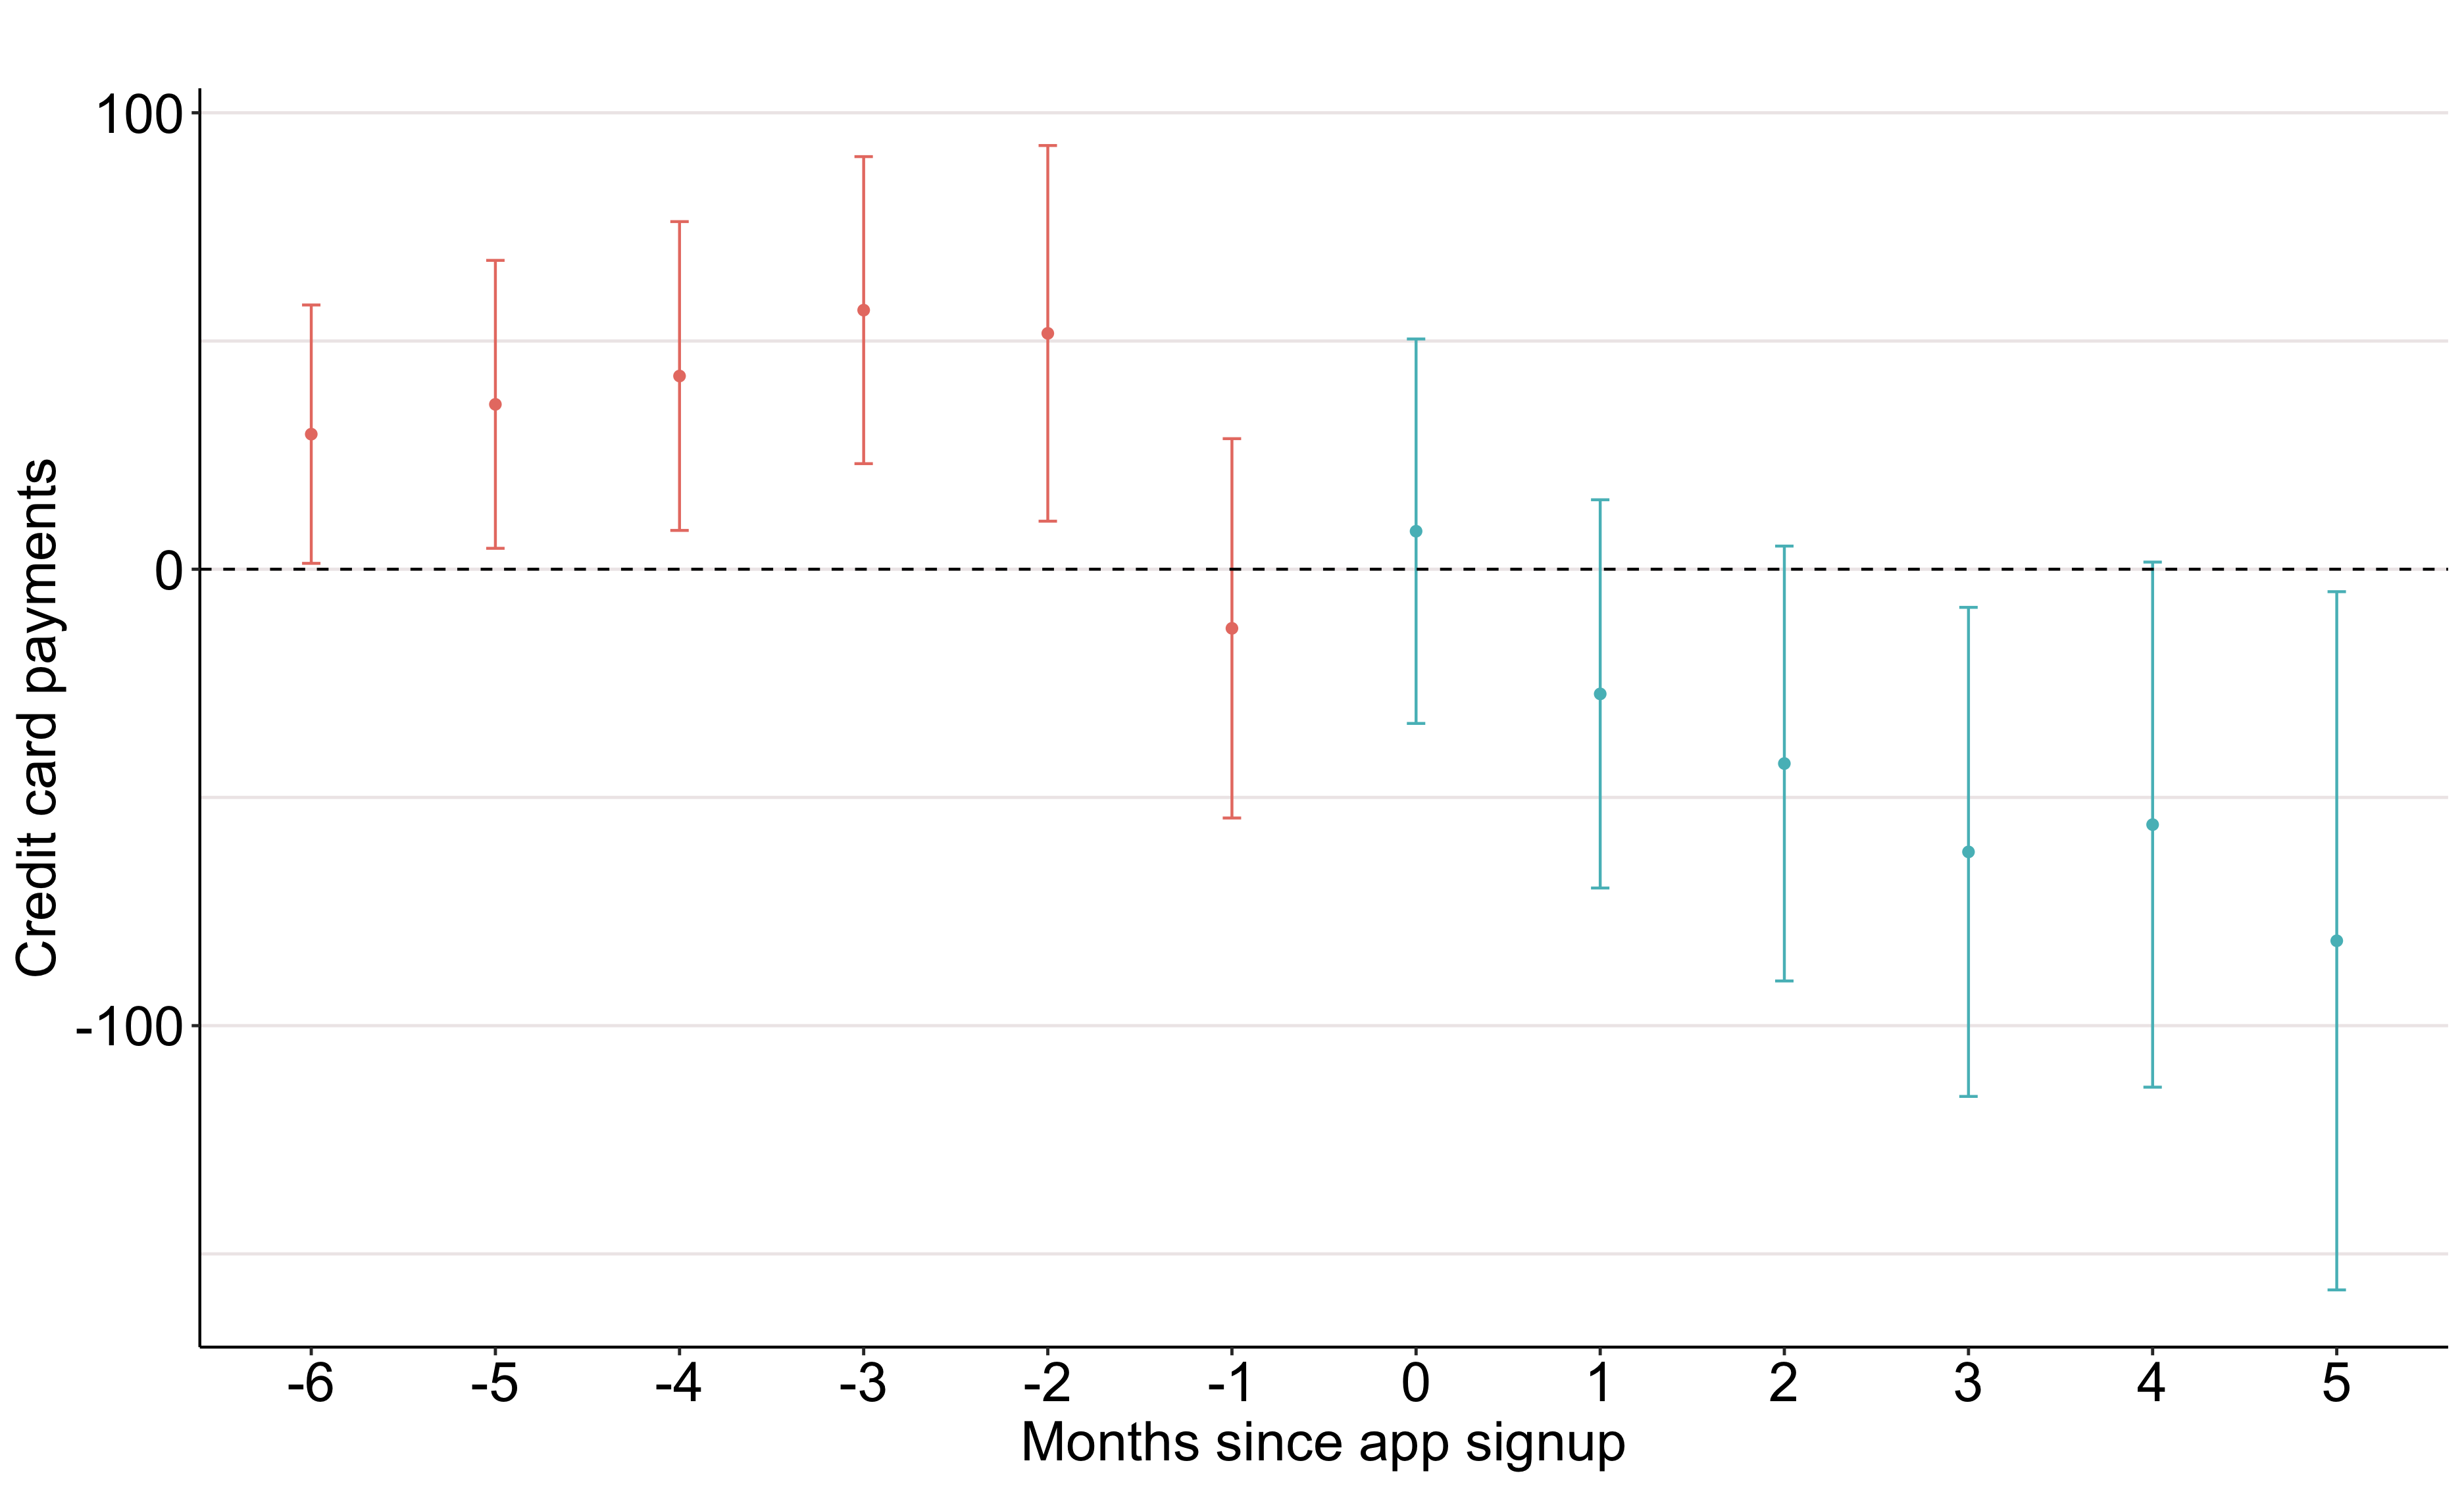
\includegraphics[width=.49\textwidth]{\figdir/cc_payments_cond_es.png}
    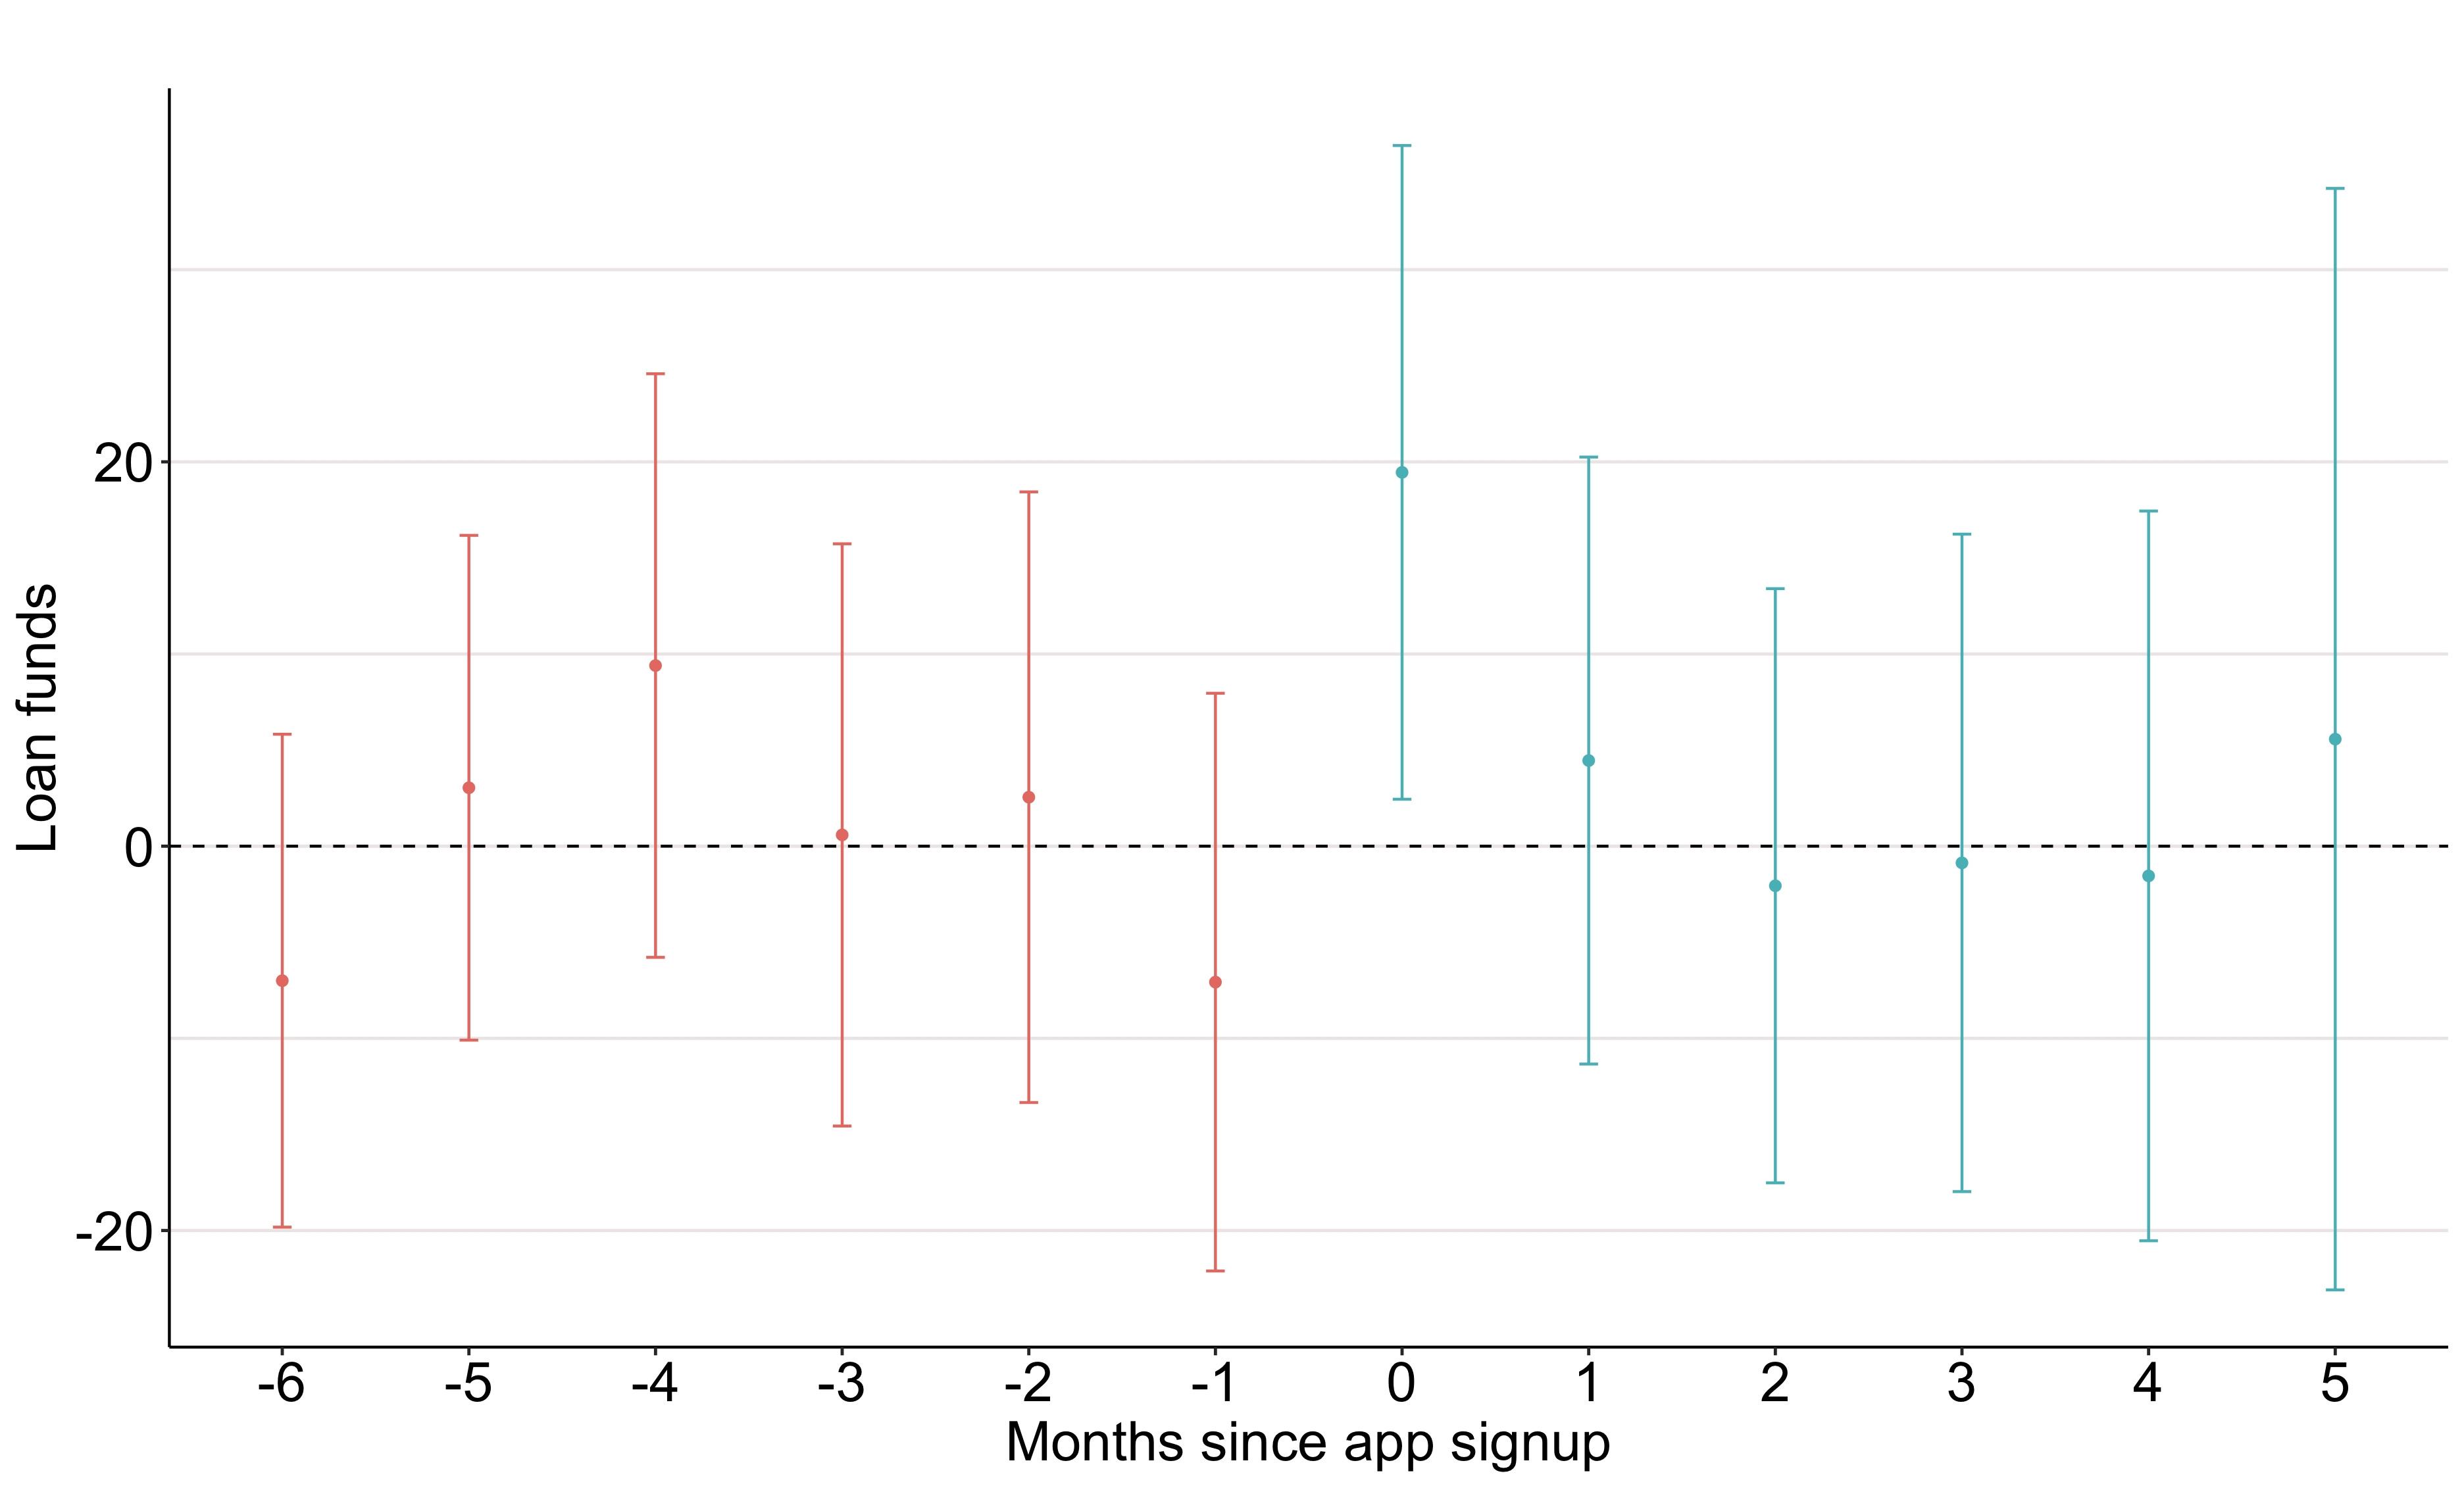
\includegraphics[width=.49\textwidth]{\figdir/loan_funds_cond_es.png}
    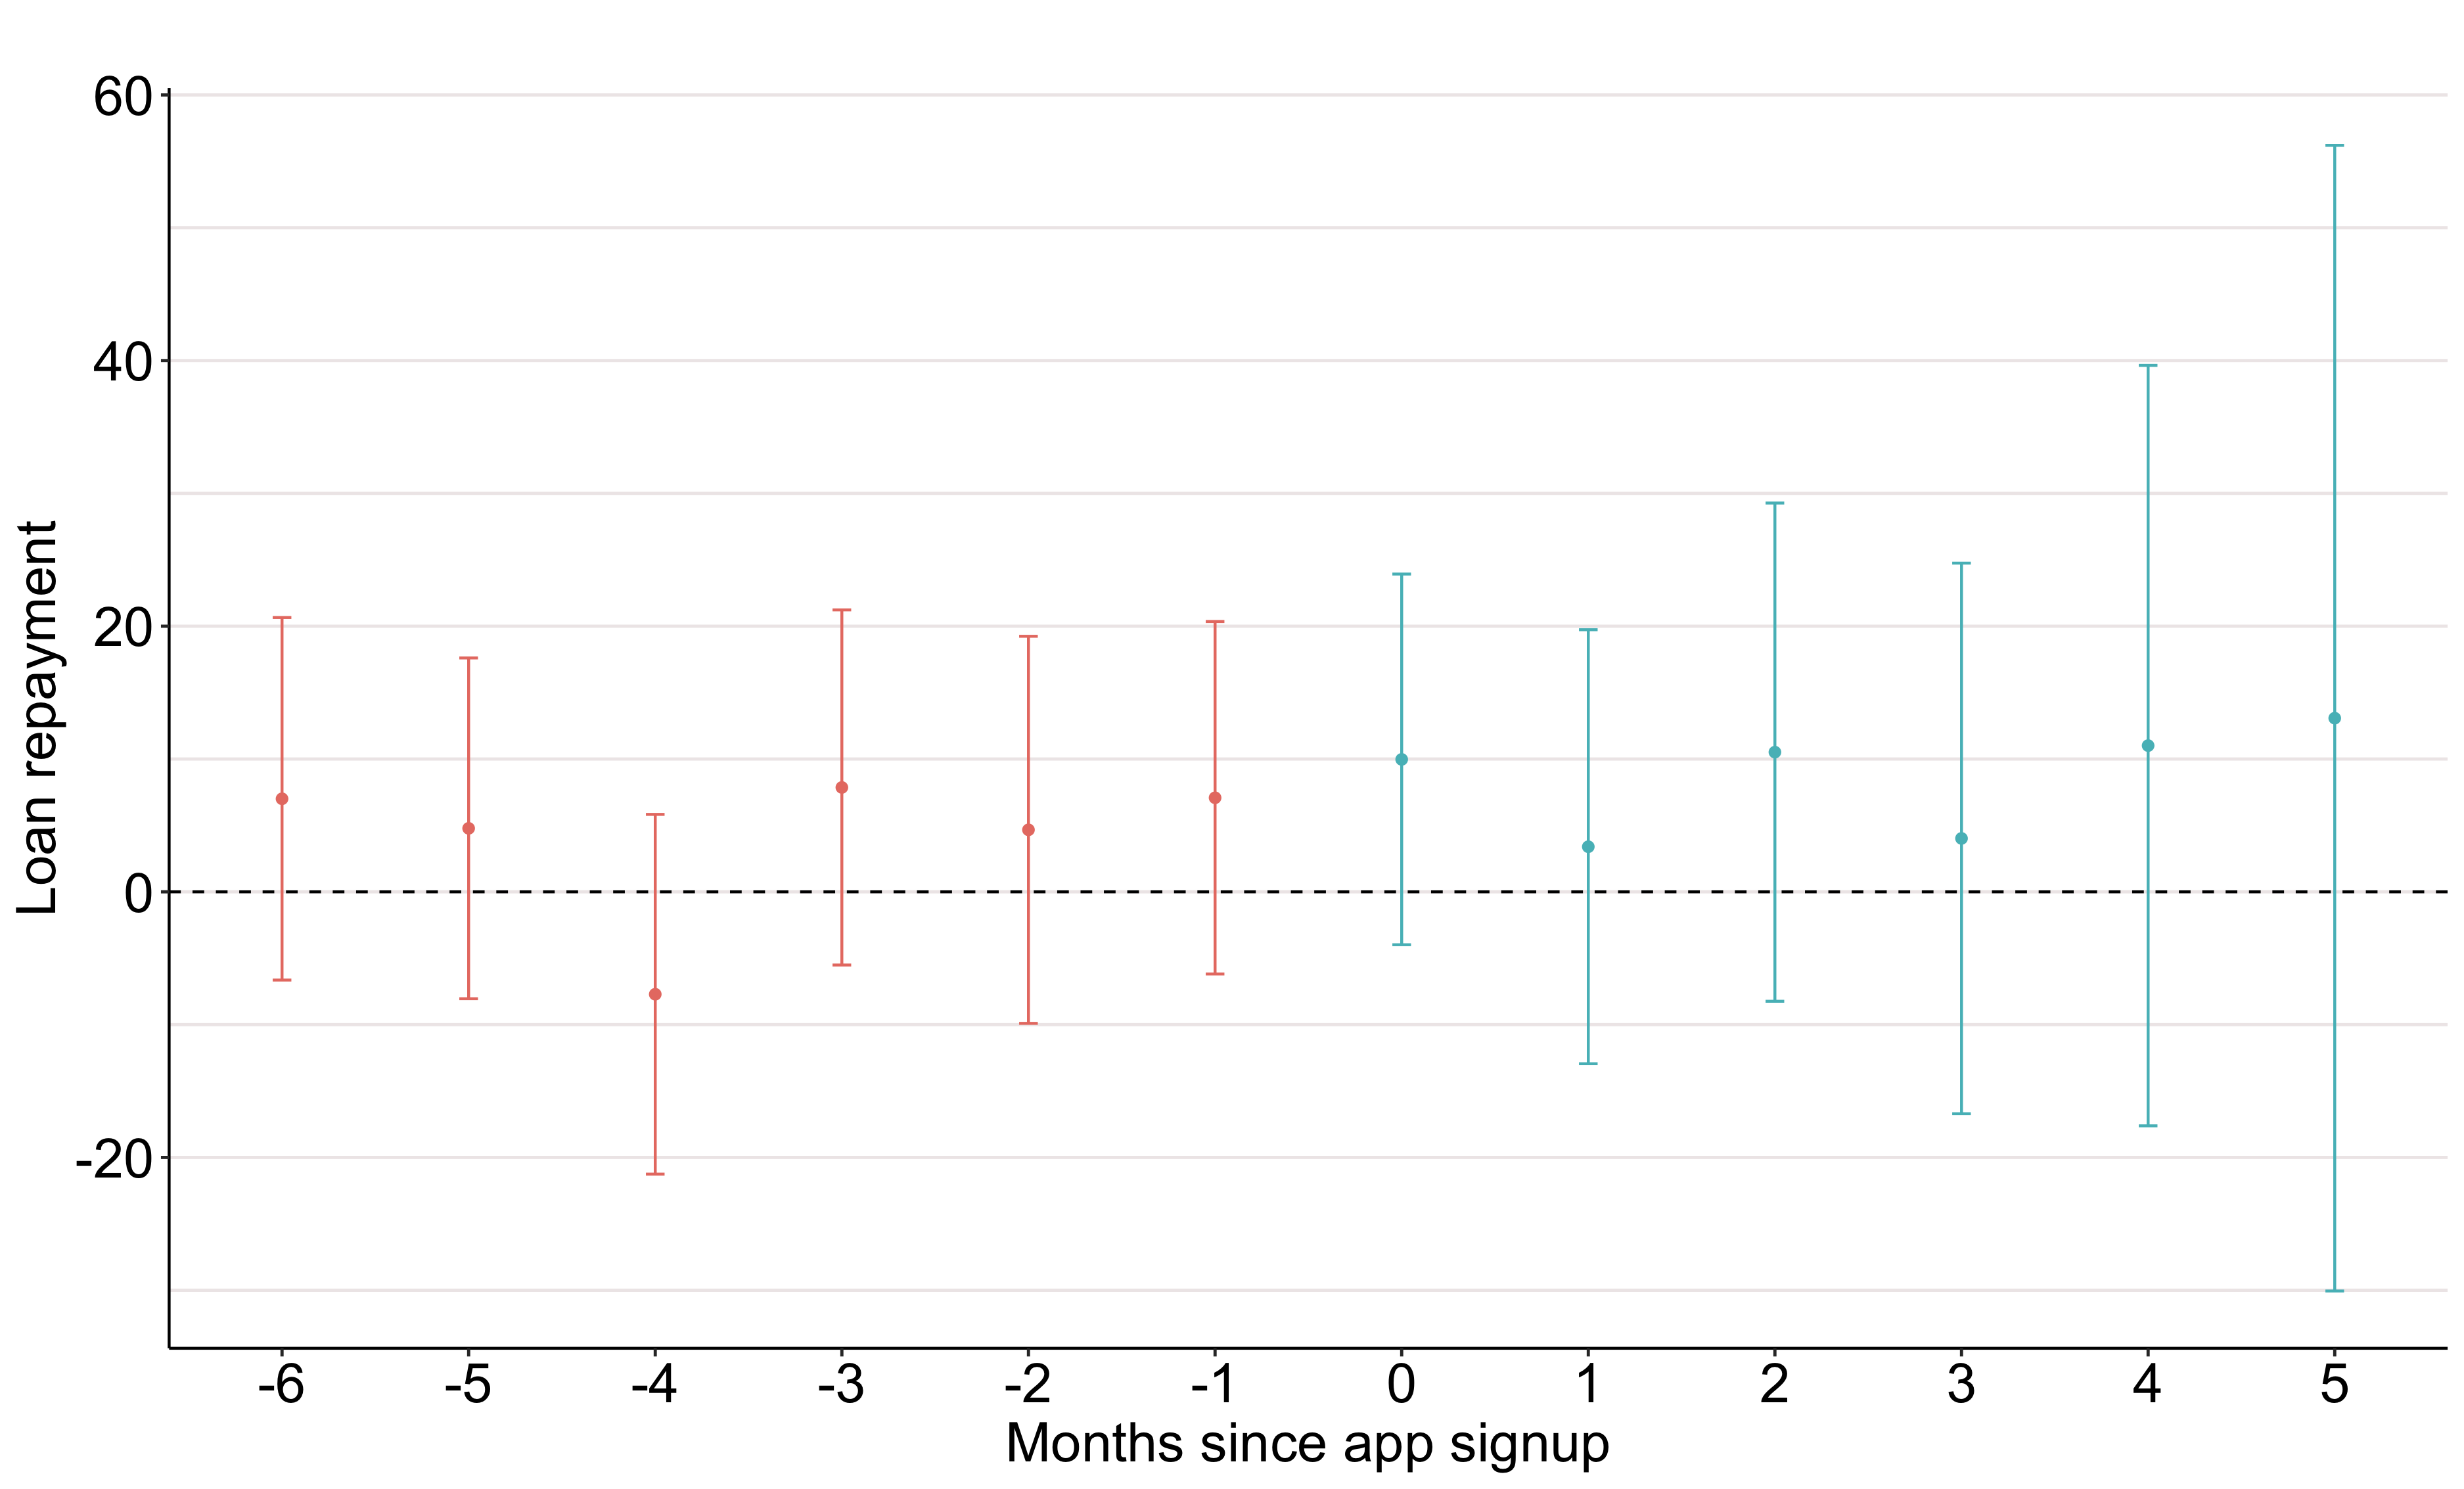
\includegraphics[width=.49\textwidth]{\figdir/loan_rpmts_cond_es.png}
    \fignote{\textwidth}{Point estimates represent
        group-time average treatment effects aggregated to periods since
        treatment exposure, as defined in Section~\ref{sub:estimation}. Red
        lines represent point estimates and uniform 95\% confidence bands for
        pre-treatment periods allowing for clustering at the user level. If the
        null hypothesis that parallel trends hold in all periods is correct,
        these should be equal to zero. Blue lines provide similar information
    for post-treatment periods.}
\end{figure}


\subsection{Subgroups}%
\label{sub:subgroups}

\begin{itemize}
    \item Look at results by subgropus (run models seperately)
\end{itemize}


